\documentclass[../master]{subfiles}

%\graphicspath{{../eps/}}

\begin{document}

\chapter{iso-C$_{\text 4}$H$_{\text{10}}$(10) + H$_{\text 2}$(9)のガス特性}
本章では検出ガスとして用いるiso-$\rm C_{4}H_{10} (1) + H_{2} (9)$の特性について述べる.
\section{ドリフトスピード}
ドリフトスピードのドリフト電場依存性を調べた.
plate, grid間の電場を3.25 V/mm -- 10.4 V/mm の間で変化させた.
線源を用いて測定したドリフトスピードとMagboltz により求めたドリフトスピードを図\ref{fig::drift_speed_E_dep}に示す.
\begin{figure}
  \centering
  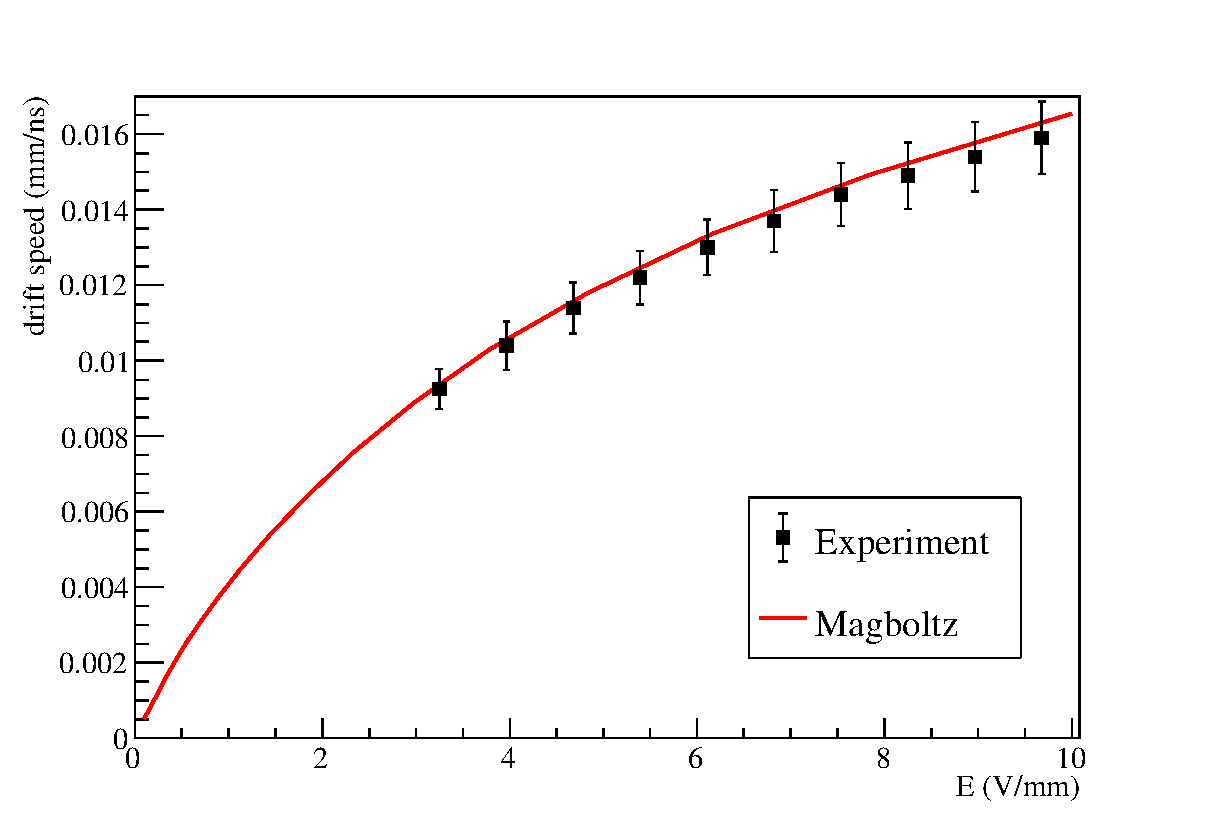
\includegraphics[clip, width=0.8\columnwidth]{drift_E_dep.eps}
  \caption{ドリフトスピードの}
  \label{fig::drift_speed_E_dep}
\end{figure}
線源を用いて測定したドリフトスピードと Magboltz で求めたドリフトスピードがおよそ一致していることが分かる.
ただ,全体的に測定値のドリフトスピードの方が小さくなている.
これは測定で用いた検出ガスに水などの不純物が含まれていることが原因と考えられる.

\section{電子増幅率}
電子の増幅率はGEM, $\mu$-PICの電圧によって変化する.
また,gridやGEMを通過する際に電子の一部が増幅されずに吸収されてしまう.
そこで,表\ref{tab::voltage_configuration}にあるような電圧を基準として電子像福利の電圧依存性を調べた.
\begin{table}
  \centering
  \caption{基準となる電圧構成.}
  \label{tab::voltage_configuration}
  \begin{tabular}{cc}
    \toprule
    & 電圧 (V)\\
    \midrule
    plate & -2255 \\
    grid & -1300 \\
    GEM (top) & -600 \\
    GEM (bottom) & -250 \\
    $\mu$-PIC & 400\\
    \bottomrule 
  \end{tabular}
\end{table}
ここで,GEMのうちgrid側をtop, $\mu$-PIC側をbottomと呼ぶ.

\subsection{GEMによる電子増幅率}
GEM は絶縁体のフィルムの両面を銅で被覆し,微細な穴を開けたものである.
GEMの各面に電圧をかけることで高電場を形成し,電子のアバランシェ増幅を起こす.
両面にかける電圧を変化させることで電子の増幅率が変化する.
GEMの両面の電位差を$\Delta V_{\rm GEM}$とすると,増幅率の電位差依存性は図\ref{fig::gain_GEM_V_dep}に示す.
\begin{figure}
  \centering
  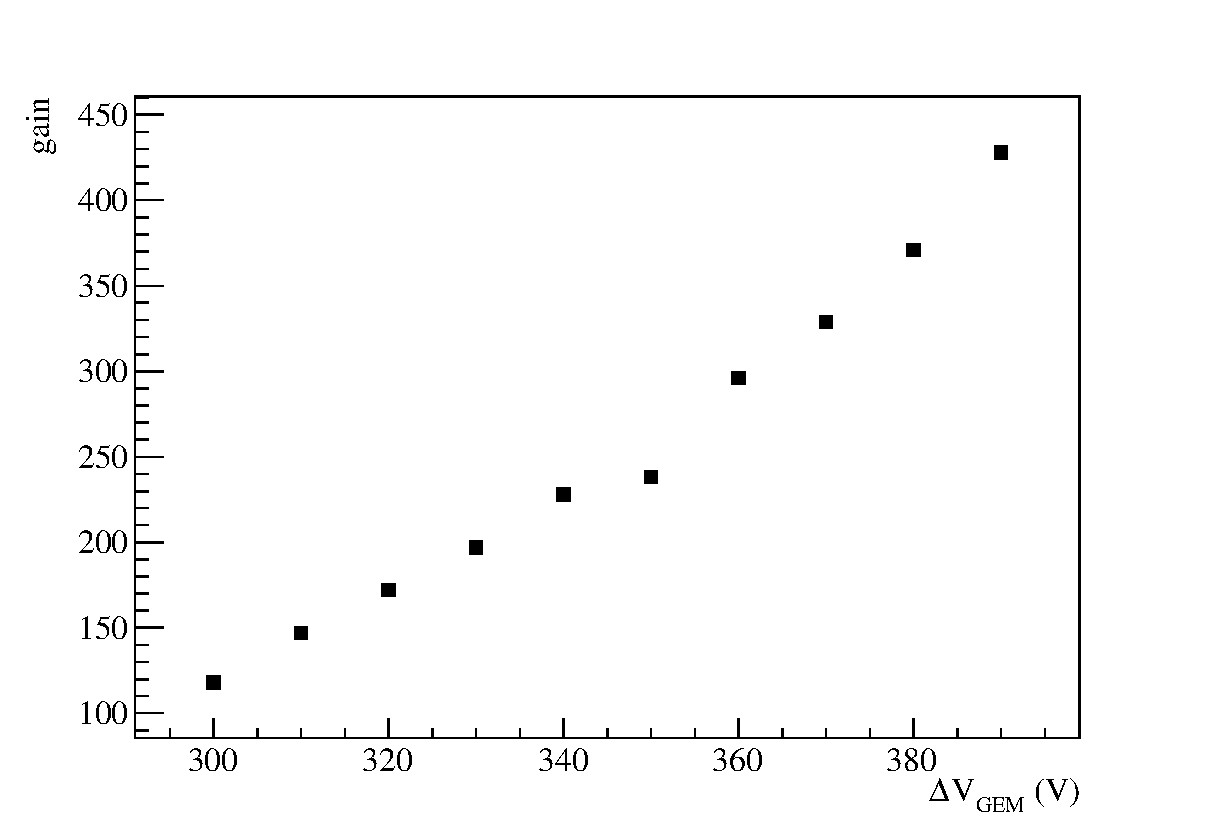
\includegraphics[clip, width=0.8\columnwidth]{gain_GEM_V_dep.eps}
  \caption{電子増幅率の$\Delta V_{\rm GEM}$依存性.}
  \label{fig::gain_GEM_V_dep}
\end{figure}
$\Delta V_{\rm GEM}$に対して増幅率が単調に増加していることが分かる.
$\Delta V_{\rm GEM} = 350 {\rm V}$とそれ以外では測定するタイミングが2時間ほどずれている.
そのため,図\ref{fig::gain_GEM_V_dep}で$V_{\rm GEM} = 350 {\rm V}$のみ不連続に変化している.

\subsection{$\mu$-PICによる電子増幅率}
電子は$\mu$-PICで読み出される直前に,$\mu$-PICによって作られた高電場によって増幅される.
$\mu$-PICのanode電極にかける電圧 ($V_{\rm\mu-PIC}$) に対する依存性を図\ref{fig::gain_uPIC_V_dep}に示す.
\begin{figure}
  \centering
  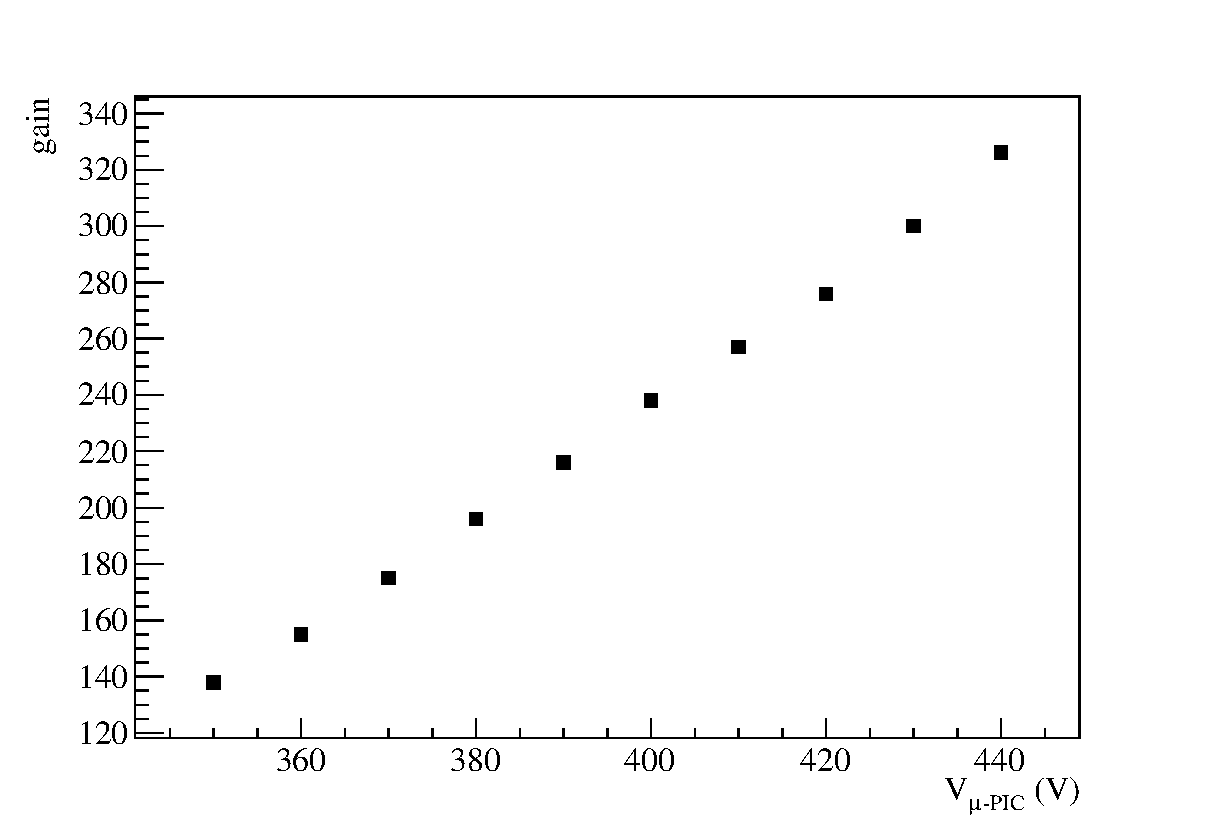
\includegraphics[clip, width=0.8\columnwidth]{gain_uPIC_V_dep.eps}
  \caption{電子増幅率の$V_{\rm\mu-PIC}$依存性.}
  \label{fig::gain_uPIC_V_dep}
\end{figure}
$V_{\rm\mu-PIC}$に対して増幅率が単調に増加していることが分かる.
GEMによる増幅率と異なり,$\mu$-PICの電圧依存性はほぼ同時に測定したため,
図\ref{fig::gain_GEM_V_dep}に見られたような不連続性は見られない.

\subsection{gridとGEM間の電位差による電子の増幅率}
gridとGEMの間の電位差によって電子がドリフト領域から増幅領域へ移動する効率が変化することがわかっている~\cite{furuno}.
最終的に得られる電子の増幅率のgridとGEMの間の電位差 ($\Delta V_{\rm grid-GEM}$) 依存性を
図\ref{fig::gain_grid_GEM_V_dep}に示す.
\begin{figure}
  \centering
  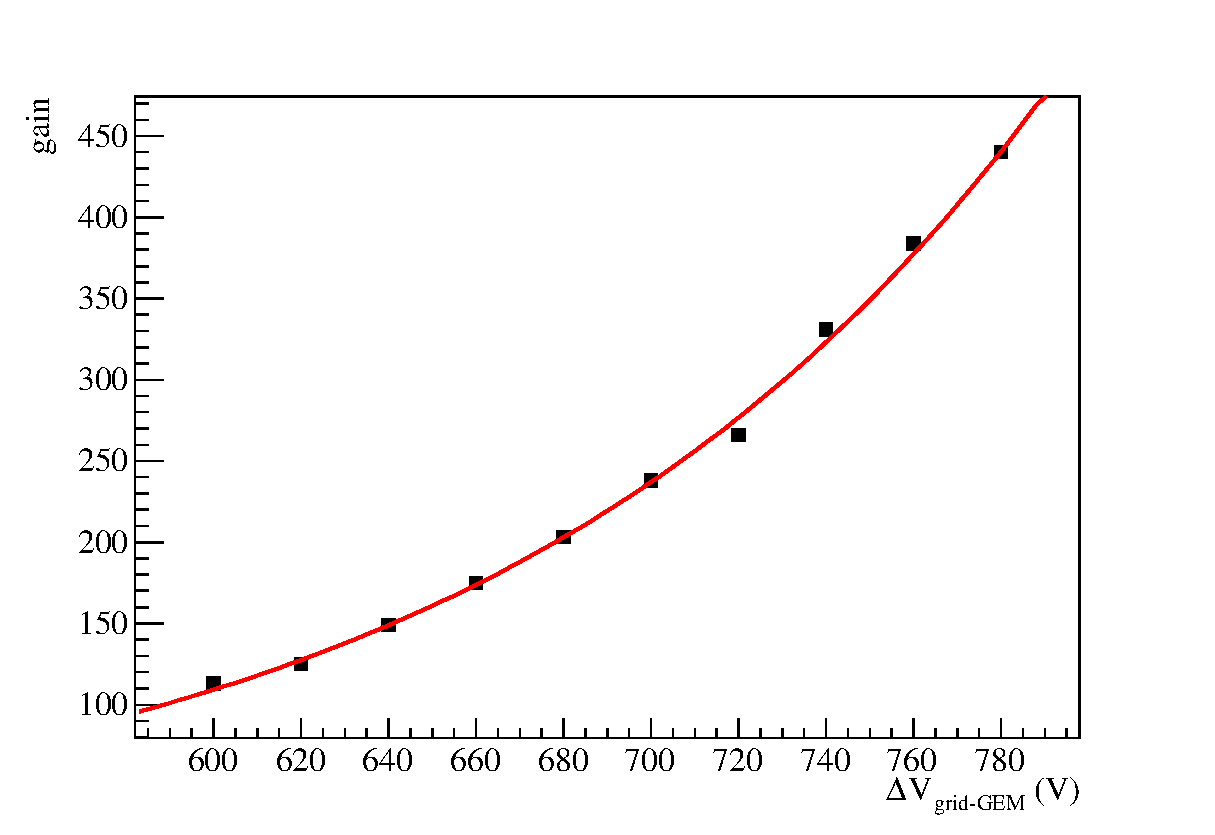
\includegraphics[clip, width=0.8\columnwidth]{gain_grid_V_dep_fit.eps}
  \caption{電子増幅率の$\Delta V_{\rm grid-GEM}$依存性.}
  \label{fig::gain_grid_GEM_V_dep}
\end{figure}
$\Delta V_{\rm grid-GEM}$にたいして増幅率が単調に増幅していることが分かる.
依存性は$4.27\times 10^{-2}\times \exp(7.75\times 10^{-3}\times \Delta V_{\rm grid-GEM})$でフィットできる.
図\ref{fig::gain_GEM_V_dep}と同様に$\Delta V_{\rm grid-GEM} = 720 {\rm V}$で不連続性が見られる.
これは,1時間ほどの時間のズレがあるためである.

\section{ディフュージョン}

%\subsection{ドリフトスピードの時間安定性}
%低圧では露点などの不純物が混ざることによって、ドリフトスピードが変化することが懸念される。
%そこで、ドリフトスピードの時間安定性の測定を行った。
%この測定は$\rm CH_{4}$ 50 hPa で行った。

\end{document}
